\def\stitle{\theexercise\ - Schleifen 1}
\section{\stitle}
\begin{frame}[t]%
    \frametitle{\stitle}
\medskip

Gegeben sei der folgende Ausschnitt eines Java-Programms.
\lstinputlisting[style=JAVAlines]{schleifen-1/Schleifen1.java}
\begin{itemize}
\item[(a)] Welche Zahl wird auf dem Bildschirm ausgegeben?
\item[(b)] Realisieren Sie diesen Programmausschnitt mit einer \code{while}-Schleife.
\end{itemize}

\end{frame}


\begin{frame}[fragile]%
 \frametitle{a) Starte Programm}%

\begin{description}[style=BASH]
\item[Konsole]
\item javac Schleifen1.java
\item java Schleifen1
\item 0  --  0
\item 1  --  1
\item 2  --  3
\item 3  --  6
\item 5  --  11
\item 6  --  17
\item Ergebnis 17
\end{description}

\begin{center}
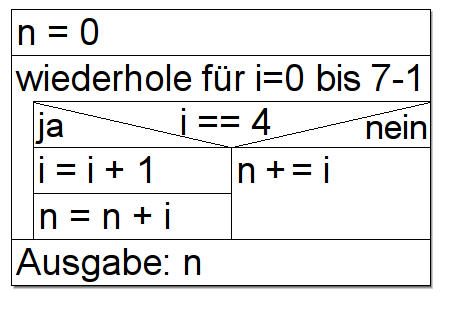
\includegraphics[width=0.5\textwidth]{schleifen-1/Bilder/Struktogramm}
\end{center}
\end{frame}


\begin{frame}[fragile]%
 \frametitle{b) Als \code{while} Schleife}%

\lstinputlisting[style=JAVAlines]{schleifen-1/Schleifen1_while.java}
\end{frame}
